\documentclass[11pt,a4paper]{article}

% ---- 中文支持（XeTeX + ctex，显式指定系统中文字体）----
\usepackage[fontset=none]{ctex}
\setCJKmainfont{Noto Serif CJK SC}
\setCJKsansfont{Noto Sans CJK SC}
\setCJKmonofont{Noto Sans CJK SC}

% ---- 排版与工具包 ----
\usepackage[a4paper,margin=2.4cm]{geometry}
\usepackage{graphicx}
\usepackage{booktabs}
\usepackage{array}
\usepackage{xcolor}
\usepackage{amsmath}
\usepackage{enumitem}
\usepackage{hyperref}
\hypersetup{colorlinks=true,linkcolor=blue,urlcolor=teal,citecolor=teal}

\definecolor{cropgreen}{RGB}{0,150,60}
\definecolor{weedred}{RGB}{200,30,30}
\definecolor{avoidred}{RGB}{180,40,40}

\setlength{\parindent}{0pt}
\setlength{\parskip}{0.5em}

\title{\bfseries 杂草检测与激光除草系统\\[0.3em] \Large 方案设计报告}
\author{农田激光除草项目组}
\date{2026年8月24日}

\begin{document}

\maketitle
\vspace{-2em}

\begin{abstract}
本报告给出农田场景下\textbf{实时杂草检测与精准激光除草}系统的完整技术方案：以 YOLO11 为目标检测基座，输出杂草框与\textbf{茎部切割线}；通过「作物轮廓 mask 膨胀 + 相交消除」的确定性后处理保证\textbf{不误伤农作物}。在公开数据集 CropAndWeed 上完成端到端验证：检测模型 mAP@0.5 达 \textbf{0.808}、推理 \textbf{99.4 FPS}，并给出带安全切割线的可视化样例。
\end{abstract}

\tableofcontents
\newpage

% ======================================================================
\section{项目目标}

在农田真实场景中，实时检测杂草，输出\textbf{杂草茎部的切割线位置}（短线段），供激光执行机构精确打击杂草茎部，实现精准除草，同时满足\textbf{不得误伤农作物}的硬约束。

\section{核心需求指标}

\begin{table}[h]
\centering
\begin{tabular}{ll}
\toprule
\textbf{指标} & \textbf{要求} \\
\midrule
帧率 & $\ge 30$ FPS \\
精度 & 高（真实光照 / 密集 / 遮挡） \\
输出 & 杂草茎部切割线（线段） \\
硬约束 & 不得误伤农作物 \\
\bottomrule
\end{tabular}
\end{table}

% ======================================================================
\section{总体技术方案}

系统由「感知」与「安全决策」两部分组成，二者职责分离：

\begin{center}
\begin{tabular}{c}
\textbf{输入图像}\\
$\downarrow$\\
\textbf{感知（模型）：}杂草框 + 茎点 + 作物轮廓 mask\\
$\downarrow$\\
\textbf{安全决策（纯代码）：}茎点生成短线 $\rightarrow$ mask 膨胀 $\rightarrow$ 相交消除\\
$\downarrow$\\
\textbf{输出：}安全切割线段（文本，供激光/运动控制模块）
\end{tabular}
\end{center}

关键设计原则：\textbf{「哪里不能打」的决策用确定性代码实现，而非让神经网络去学}。模型只负责感知（看见框、茎点、轮廓），安全门控用可证明、可复现的几何规则——因为「误伤作物」是不可接受的失败模式，不能容忍模型的一次幻觉。

% ======================================================================
\section{模型选型：YOLO11}

\subsection{版本谱系}

YOLO 版本号分两条线：官方主线（Ultralytics：v5 $\to$ v8 $\to$ \textbf{YOLO11} $\to$ YOLO26）与学术衍生（v6/v7/v9/v10/v12/v13）。选择 \textbf{YOLO11}，兼顾精度、速度、生态与部署工程化，且对小目标（茎）能力适配。

\subsection{三种任务分工}

\begin{table}[h]
\centering
\begin{tabular}{lll}
\toprule
\textbf{模型} & \textbf{输出} & \textbf{用途} \\
\midrule
YOLO11 \textbf{detect} & 框 + 类别 & 定位「杂草 / 作物在哪」 \\
YOLO11 \textbf{pose} & 框 + 关键点 & 茎的\textbf{离散点}（切割线中心） \\
YOLO11 \textbf{seg} & 框 + 实例 mask & 作物\textbf{轮廓}（避让禁区） \\
\bottomrule
\end{tabular}
\end{table}

% ======================================================================
\section{切割方案：茎部短线段}

\subsection{方案对比}

\begin{table}[h]
\centering
\begin{tabular}{lll}
\toprule
\textbf{维度} & \textbf{方案1：茎离散点} & \textbf{方案2：茎位置横线} \\
\midrule
激光动作 & 精确打几个点 & 沿短线段扫描 \\
鲁棒性（茎摆动/抖动） & 低 & \textbf{高} \\
标注成本 & 贵（关键点 3--5 倍） & 便宜（框 + 一点） \\
\bottomrule
\end{tabular}
\end{table}

\textbf{采用方案2的改良版}：由茎点生成\textbf{短线段}（茎宽 $\pm$ 几毫米，\textbf{不横跨整框}），吸收茎细、随风摆动与机器人抖动带来的毫米级误差。

\subsection{本报告实现参数}

茎点两侧各延长 $20$ px，切割线总长 $40$ px（可调）。此长度由「茎宽 + 定位误差 + 摆动余量」决定，与目标框大小\textbf{无关}——框宽是整株冠幅（上百像素），茎本身只有几个像素。

% ======================================================================
\section{作物避让：mask 而非框}

\subsection{为什么不能用「框 $\cap$ 框」}

框是矩形，作物不是矩形。倾斜/稀疏作物的矩形框会盖住大片空地；杂草长在这片空地、离作物本体尚远时，框判断会误报冲突 $\to$ 激光误关 $\to$ 漏除。因此避让决策必须基于\textbf{作物轮廓 mask}。

\subsection{三层精度}

\begin{table}[h]
\centering
\begin{tabular}{lll}
\toprule
\textbf{层级} & \textbf{相交依据} & \textbf{效果} \\
\midrule
L0 & 框 $\cap$ 框 & 误报多 \\
L1 & mask $\cap$ mask & 精确 \\
\textbf{L2（采用）} & \textbf{膨胀 mask $\cap$ 线段} & \textbf{工程正解} \\
\bottomrule
\end{tabular}
\end{table}

膨胀余量 $= $ 激光光斑半径 $+$ 安全距离 $+$ 分割边缘误差 $+$ 茎摆动余量。实现上以 $3\times3$ 核迭代 $N$ 次，实现\textbf{精确 $N$ 像素膨胀}。

\subsection{处理流程}

\begin{enumerate}[label=\textbf{(\arabic*)}]
  \item 茎点生成水平短线段（含延长余量）；
  \item 作物 mask 膨胀一圈（安全余量）；
  \item 短线段与膨胀后 mask 求交，消除落在禁区内的子段；
  \item 输出剩余的安全可打线段；若整段被挡，标记为 \texttt{blocked}。
\end{enumerate}

% ======================================================================
\section{数据集：CropAndWeed}\label{sec:dataset}

\begin{itemize}[leftmargin=1.5em]
  \item 来源：CropAndWeed（WACV 2023），非商用许可，仅研究用途。
  \item 规模：\textbf{8034} 张图，$1920\times1088$ RGB；8 种作物 + 16 类杂草。
  \item 标注：框 + \textbf{茎点（StemX, StemY）} + 语义分割 mask。
  \item 转换：作物 $\to$ 0、杂草 $\to$ 1（二分类）；丢弃 label 255（模糊植被兜底类，约占总目标 40\%）。
  \item 划分：有效 \textbf{7705} 张（train 6164 / val 1541），共 78288 目标。
\end{itemize}

\textbf{茎点标注质量提示}：抽查 200 图 / 3440 目标，\textbf{69\% 的茎点几乎等于框中心}（偏移 $<2$ px）。即该数据集的「茎点」多为近似植物中心、非精确茎基部，pose 模型学到的是「框中心」级精度；真机若需毫米级切茎基部，应自标「真茎基部」关键点做微调。

% ======================================================================
\section{实验与结果}

\subsection{检测模型（detect）}

\begin{table}[h]
\centering
\begin{tabular}{lll}
\toprule
\textbf{配置} & \multicolumn{2}{l}{YOLO11n，2.59M 参数，6.4 GFLOPs} \\
 & \multicolumn{2}{l}{100 epochs，imgsz 640，batch 16，RTX 3050} \\
\midrule
\textbf{指标} & \textbf{全量 7705 图} & \textbf{子集 1739 图} \\
\midrule
mAP@0.5 & \textbf{0.808} & 0.758 \\
mAP@0.5:0.95 & \textbf{0.569} & 0.515 \\
mAP@0.75 & 0.600 & 0.540 \\
Precision & 0.787 & 0.764 \\
Recall & 0.755 & 0.720 \\
\bottomrule
\end{tabular}
\end{table}

\begin{table}[h]
\centering
\begin{tabular}{lll}
\toprule
\textbf{指标} & \textbf{数值} & \textbf{说明} \\
\midrule
FPS & \textbf{99.4} & batch=1，10.1 ms/帧 \\
目标 & 16128 & 验证集实例数 \\
\bottomrule
\end{tabular}
\end{table}

全量数据相较子集提升约 5 个点 mAP@0.5，实时性稳定保持 $\sim$100 FPS，约为 30 FPS 目标的 3 倍余量。

\subsection{姿态模型（pose，茎点）}

YOLO11n-pose，每目标 1 个关键点（茎点），$kpt\_shape=[1,3]$，用于将检测框升级为「框 + 茎点」的完整输出。训练 30 epochs 收尾版（停电截止前的降配，后续可 \texttt{resume} 续训至 100）。

\begin{table}[h]
\centering
\begin{tabular}{lll}
\toprule
\textbf{配置} & \multicolumn{2}{l}{YOLO11n-pose，30 epochs，imgsz 640，batch 16} \\
\midrule
\textbf{指标} & \textbf{数值} & \textbf{说明} \\
\midrule
关键点（茎点）mAP@0.5 & \textbf{0.841} & 茎点定位精度 \\
关键点 mAP@0.5:0.95 & \textbf{0.835} & \\
框 mAP@0.5 & 0.768 & 检测框（同 detect 量级） \\
框 mAP@0.5:0.95 & 0.524 & \\
Pose Precision & 0.788 & \\
FPS & \textbf{99.6} & 10.0 ms/帧 \\
\bottomrule
\end{tabular}
\end{table}

\textbf{注意}：关键点 mAP 0.841 高于框 mAP，是因为该数据集「茎点 $\approx$ 框中心」（见 \S\ref{sec:dataset}），模型学到的茎点精度即「框中心」级；真机若需毫米级切茎基部，应以自标「真茎基部」关键点微调。

% ======================================================================
\section{部署与输出接口}

推理链路为\textbf{多模型级联 + 确定性后处理}，非单一端到端模型：

\begin{center}
\texttt{detect/pose 模型} $\to$ \texttt{compute\_safe\_cut\_lines()} $\to$ \texttt{cuts\_to\_text()} $\to$ \textbf{下游激光/运动控制}
\end{center}

下游模块只消费坐标文本，不消费图像。输出示例（JSON）：

\begin{verbatim}
{"frame_id": 1001, "num_weeds": 2, "num_blocked": 0,
 "weeds": [
   {"id": 0, "stem": [11.0, 118.0],
    "cut_segments": [[0, 31, 118]], "blocked": false},
   {"id": 1, "stem": [724.0, 1079.0],
    "cut_segments": [[704, 744, 1079]], "blocked": false}]}
\end{verbatim}

当前坐标为\textbf{像素系}；接深度相机与\textbf{手眼标定}后升级为机器人基座系的三维坐标。

% ======================================================================
\section{测试样例}

下图为本系统在验证集上的可视化输出，图例统一为：

\begin{itemize}[leftmargin=1.5em]
  \item \textcolor{weedred}{\textbf{红色框}}：模型预测的杂草；
  \item \textcolor{cropgreen}{\textbf{绿色框}}：模型预测的作物；
  \item \textcolor{cropgreen}{\textbf{绿色短线段}}：安全切割线（40 px，落于茎点）；
  \item \textcolor{avoidred}{\textbf{红色半透明}}：作物轮廓膨胀后的禁区；
  \item \textbf{黄色框}：真实杂草框（GT）。
\end{itemize}

\begin{figure}[h]
\centering
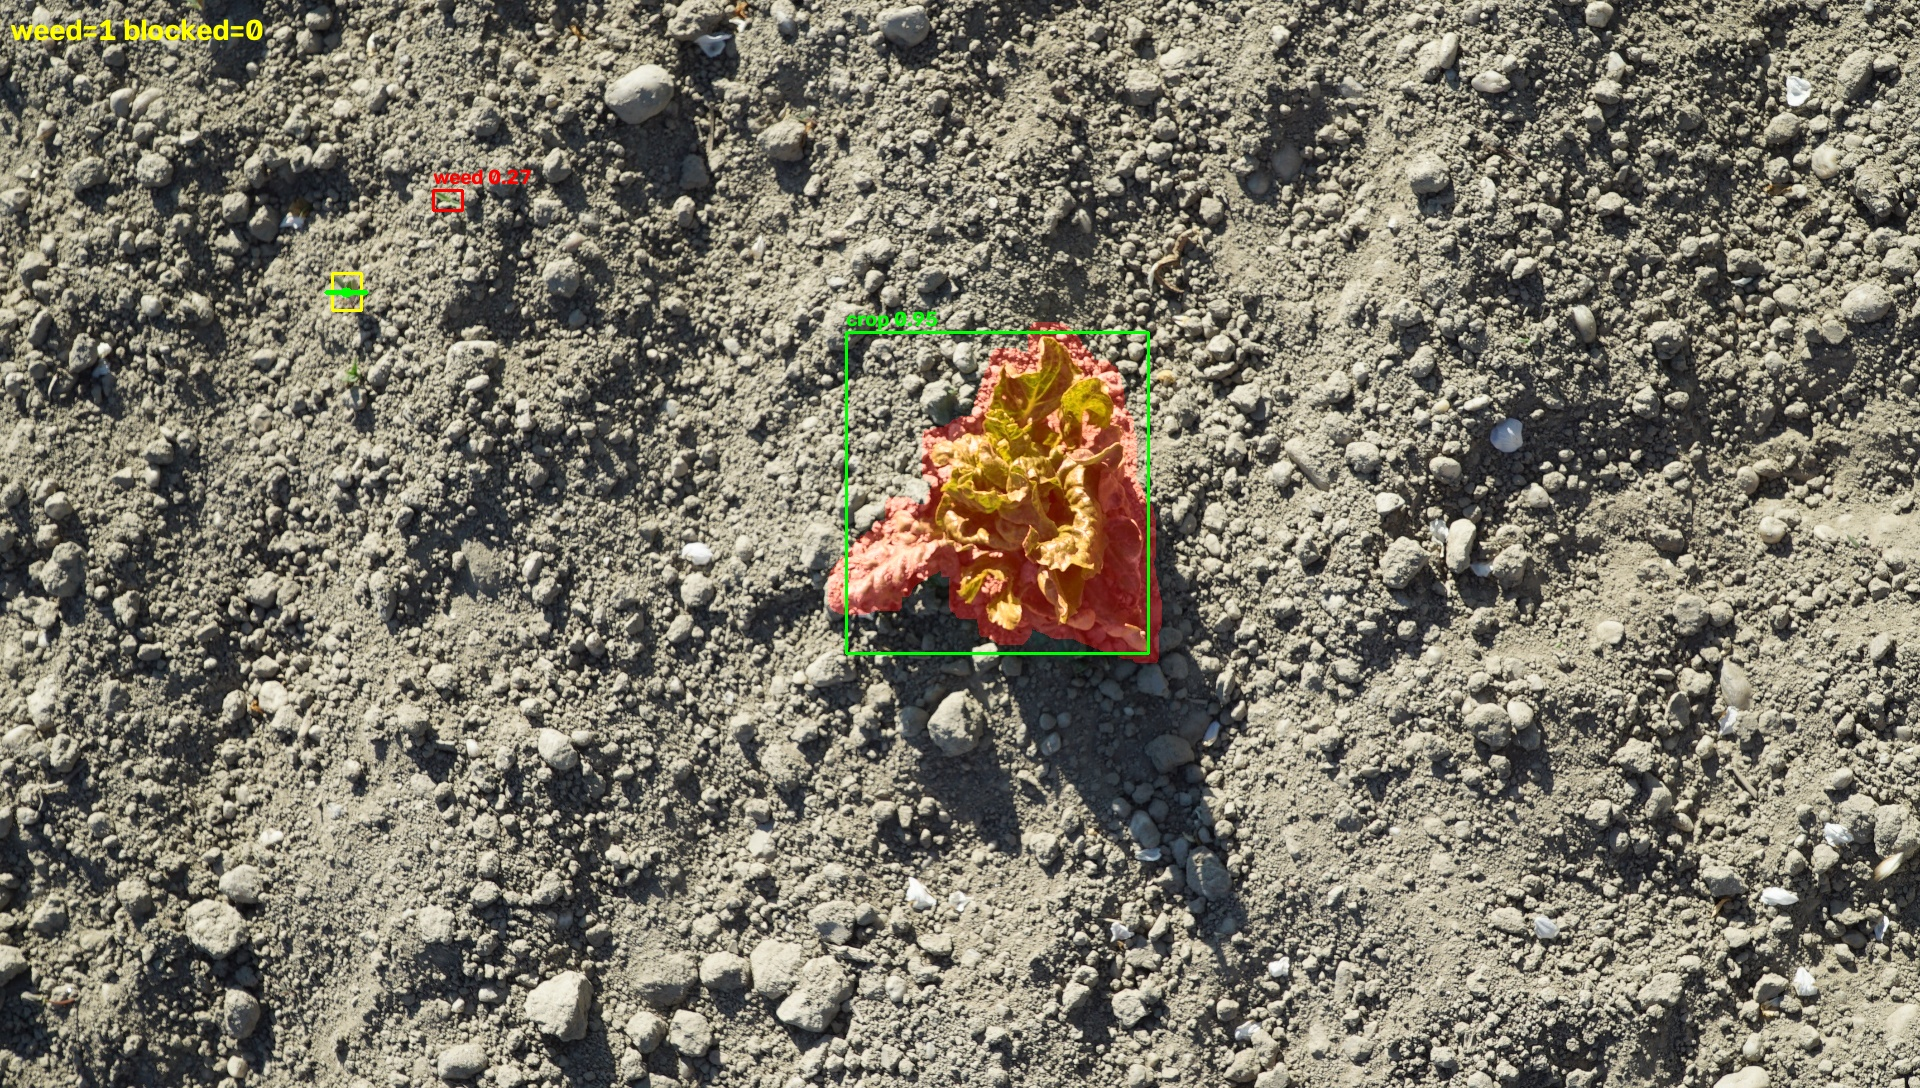
\includegraphics[width=0.88\linewidth]{images/ave-0037-0008.jpg}
\caption{单目标样例：一株杂草，框 + 茎点 + 40 px 安全切割短线。}
\end{figure}

\begin{figure}[h]
\centering
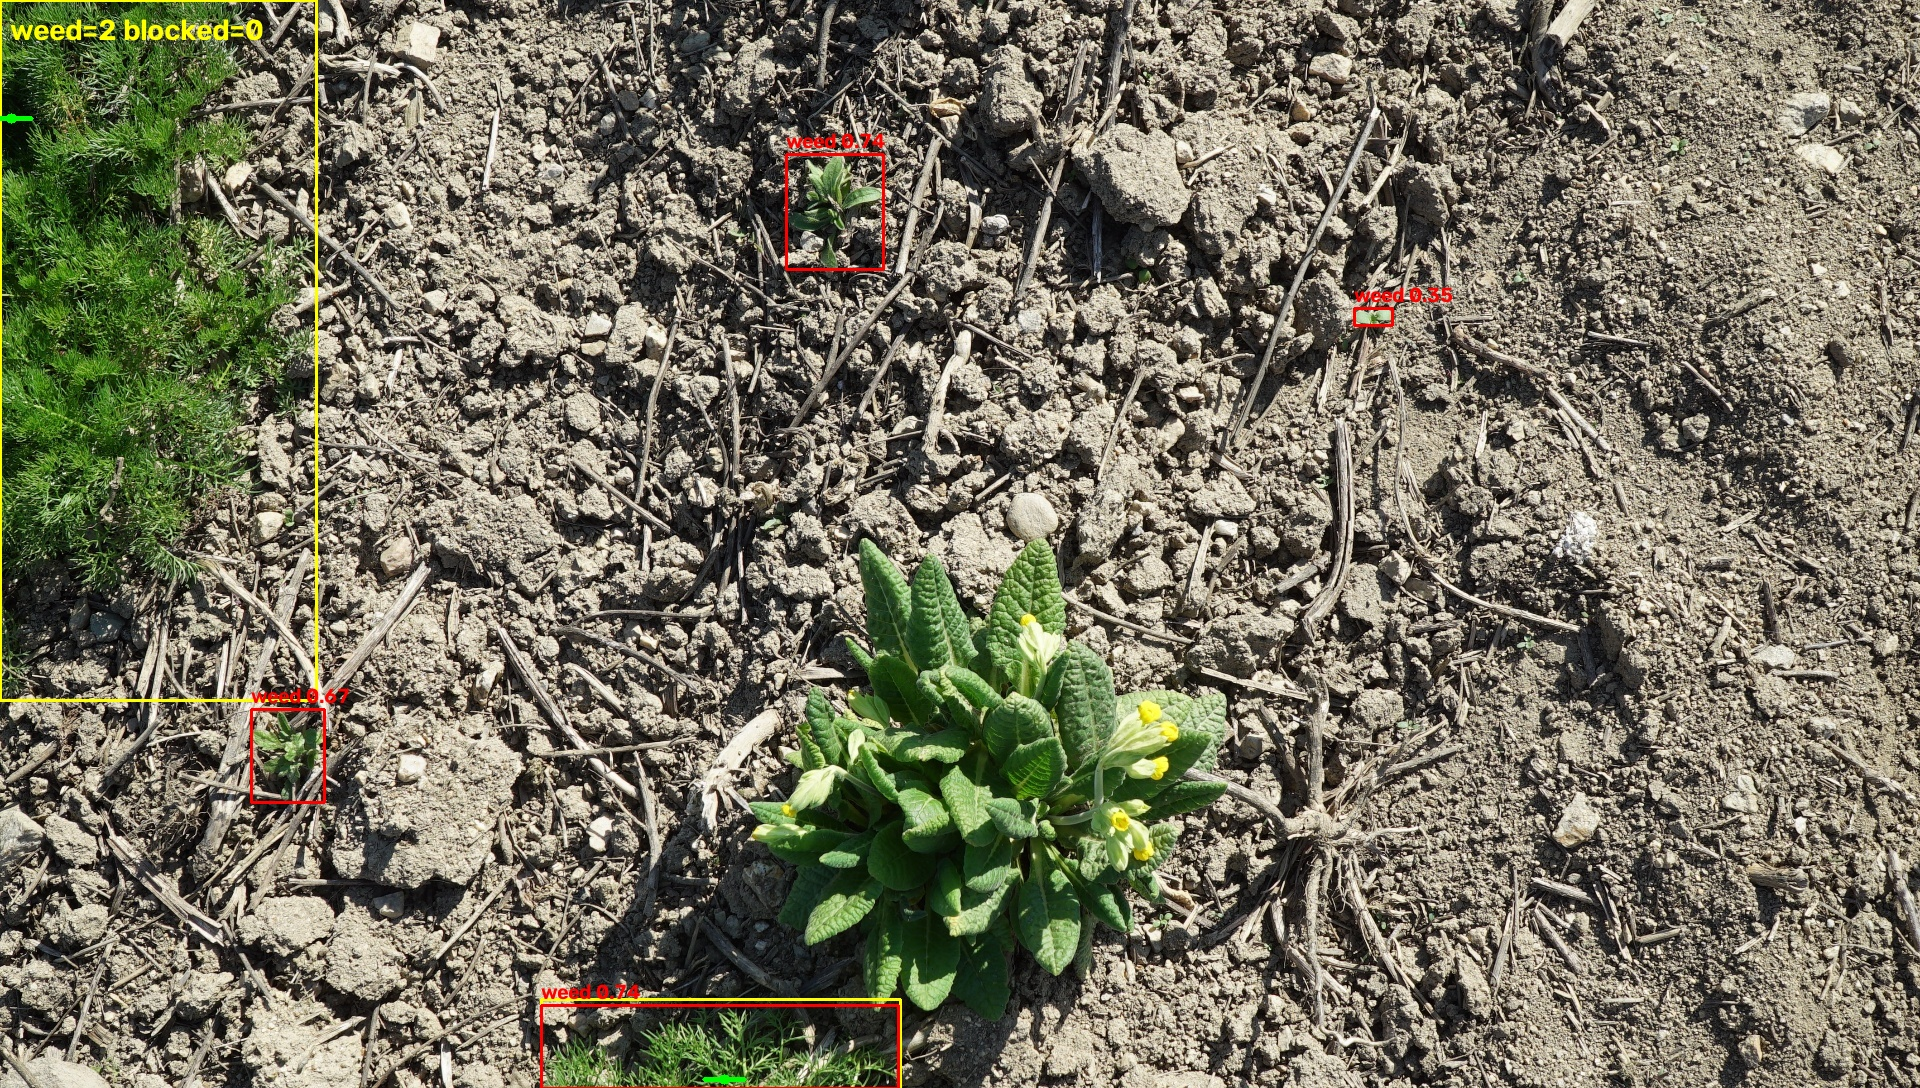
\includegraphics[width=0.88\linewidth]{images/ave-0035-0005.jpg}
\caption{双目标样例：两株杂草分别输出各自的切割短线。}
\end{figure}

\begin{figure}[h]
\centering
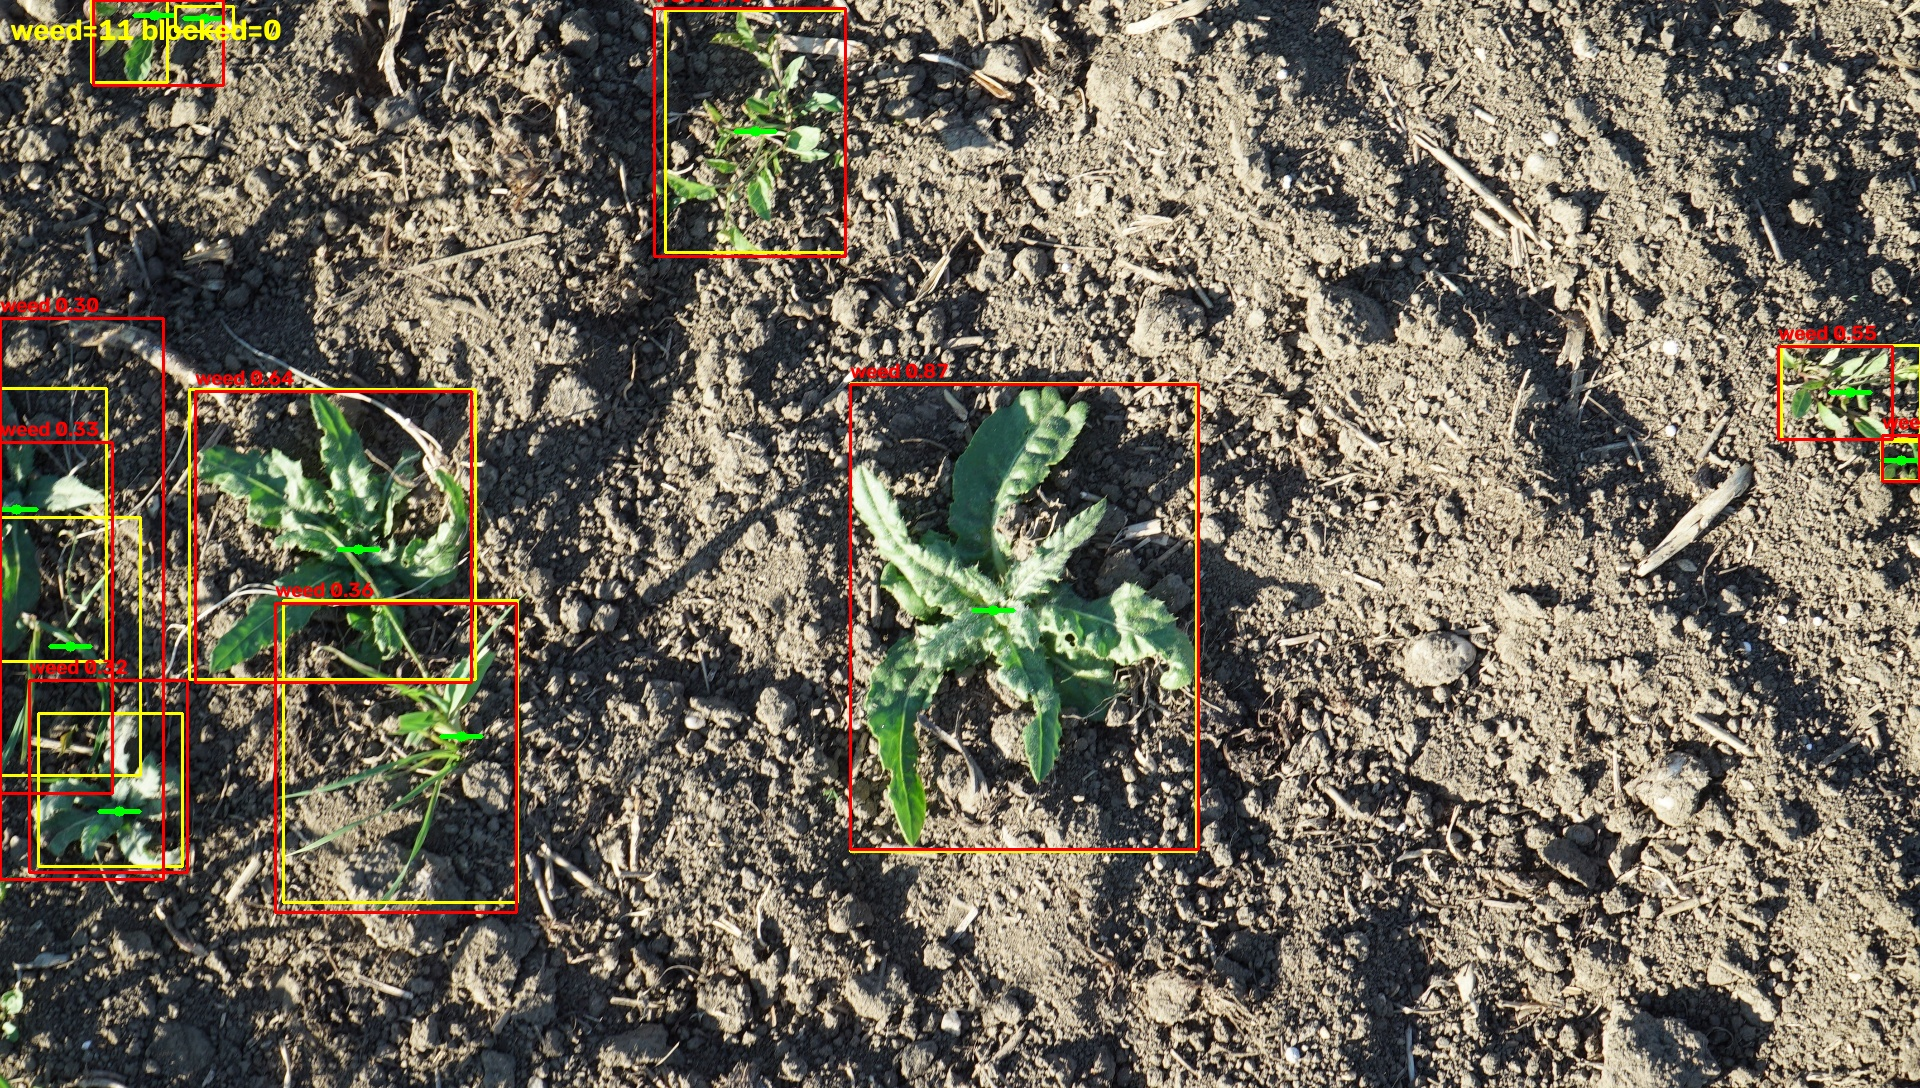
\includegraphics[width=0.88\linewidth]{images/ave-0041-0003.jpg}
\caption{较密集样例：多株杂草同时检出并输出切割线，红色禁区叠加作物区域。}
\end{figure}

\begin{figure}[h]
\centering
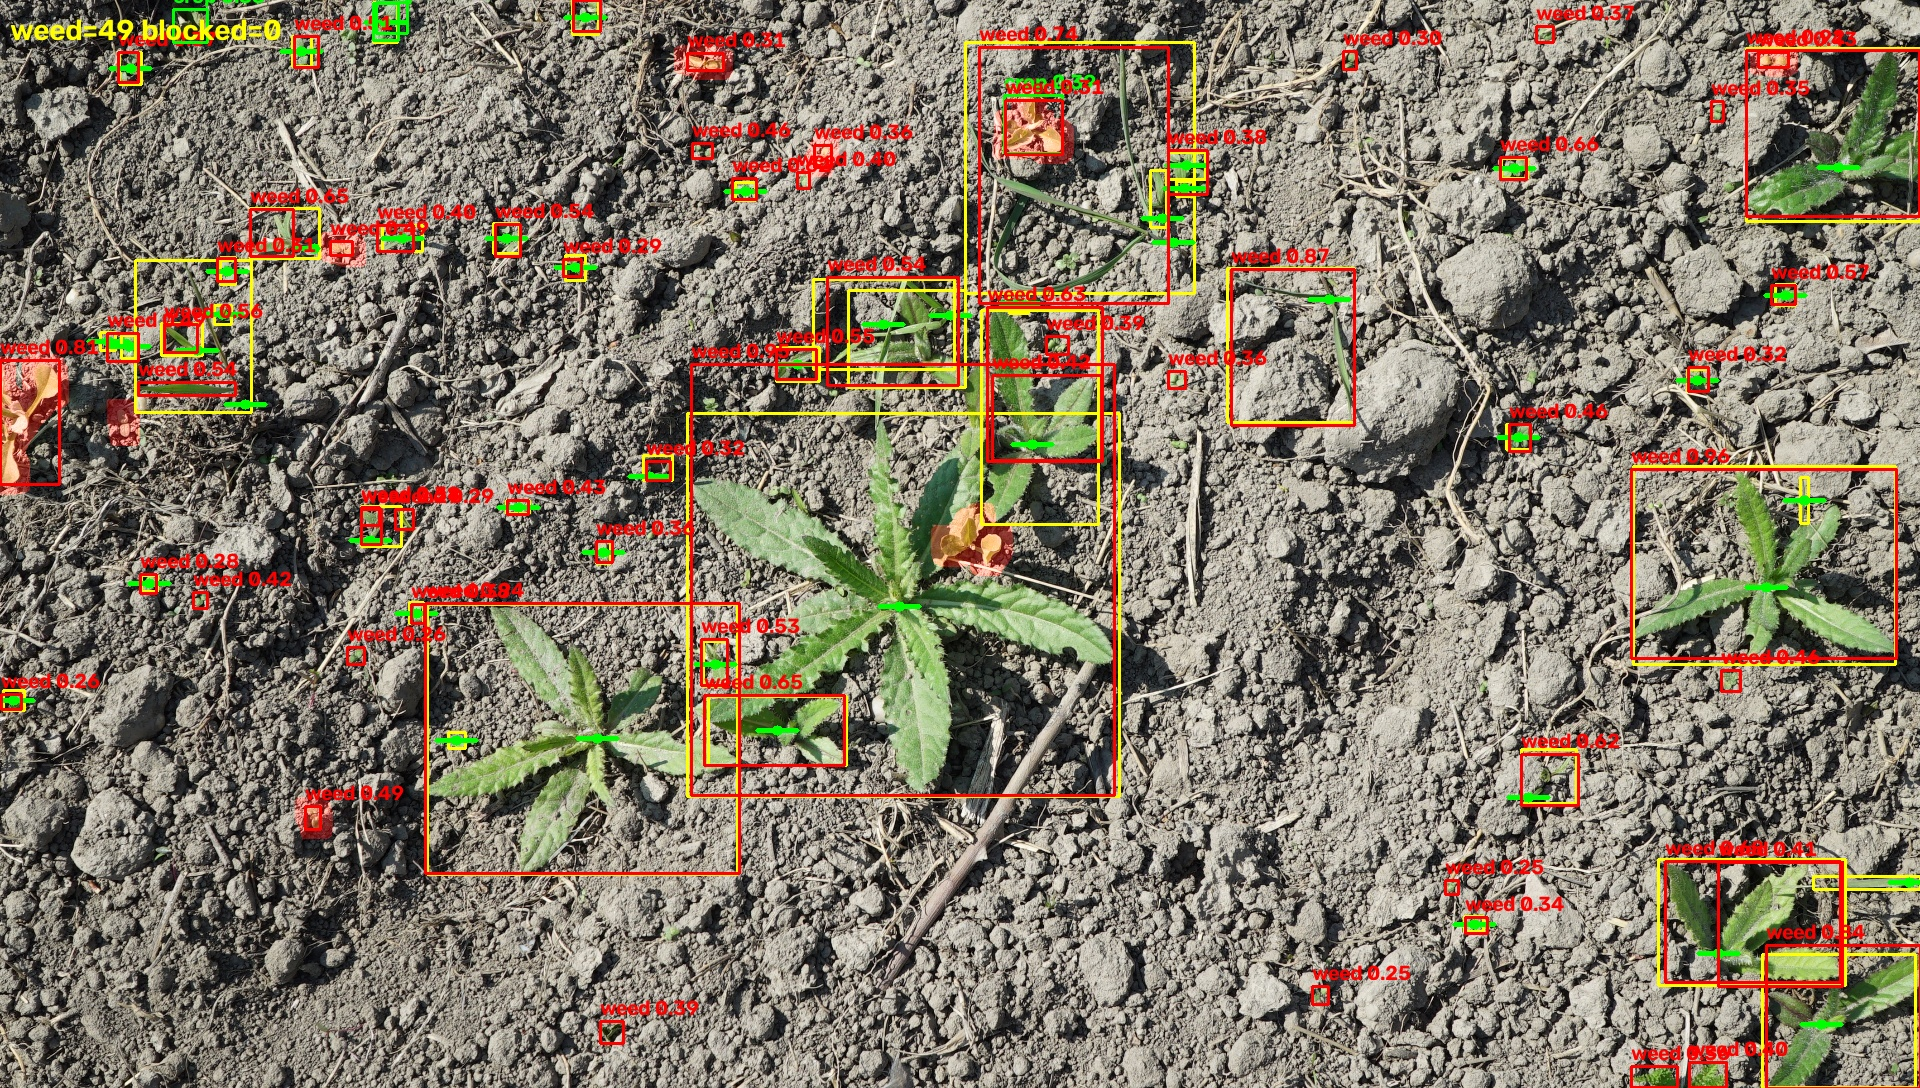
\includegraphics[width=0.88\linewidth]{images/ave-0007-0000.jpg}
\caption{高密度大田样例：整幅图像中大量杂草被检出并标注切割位置。}
\end{figure}

\begin{figure}[h]
\centering
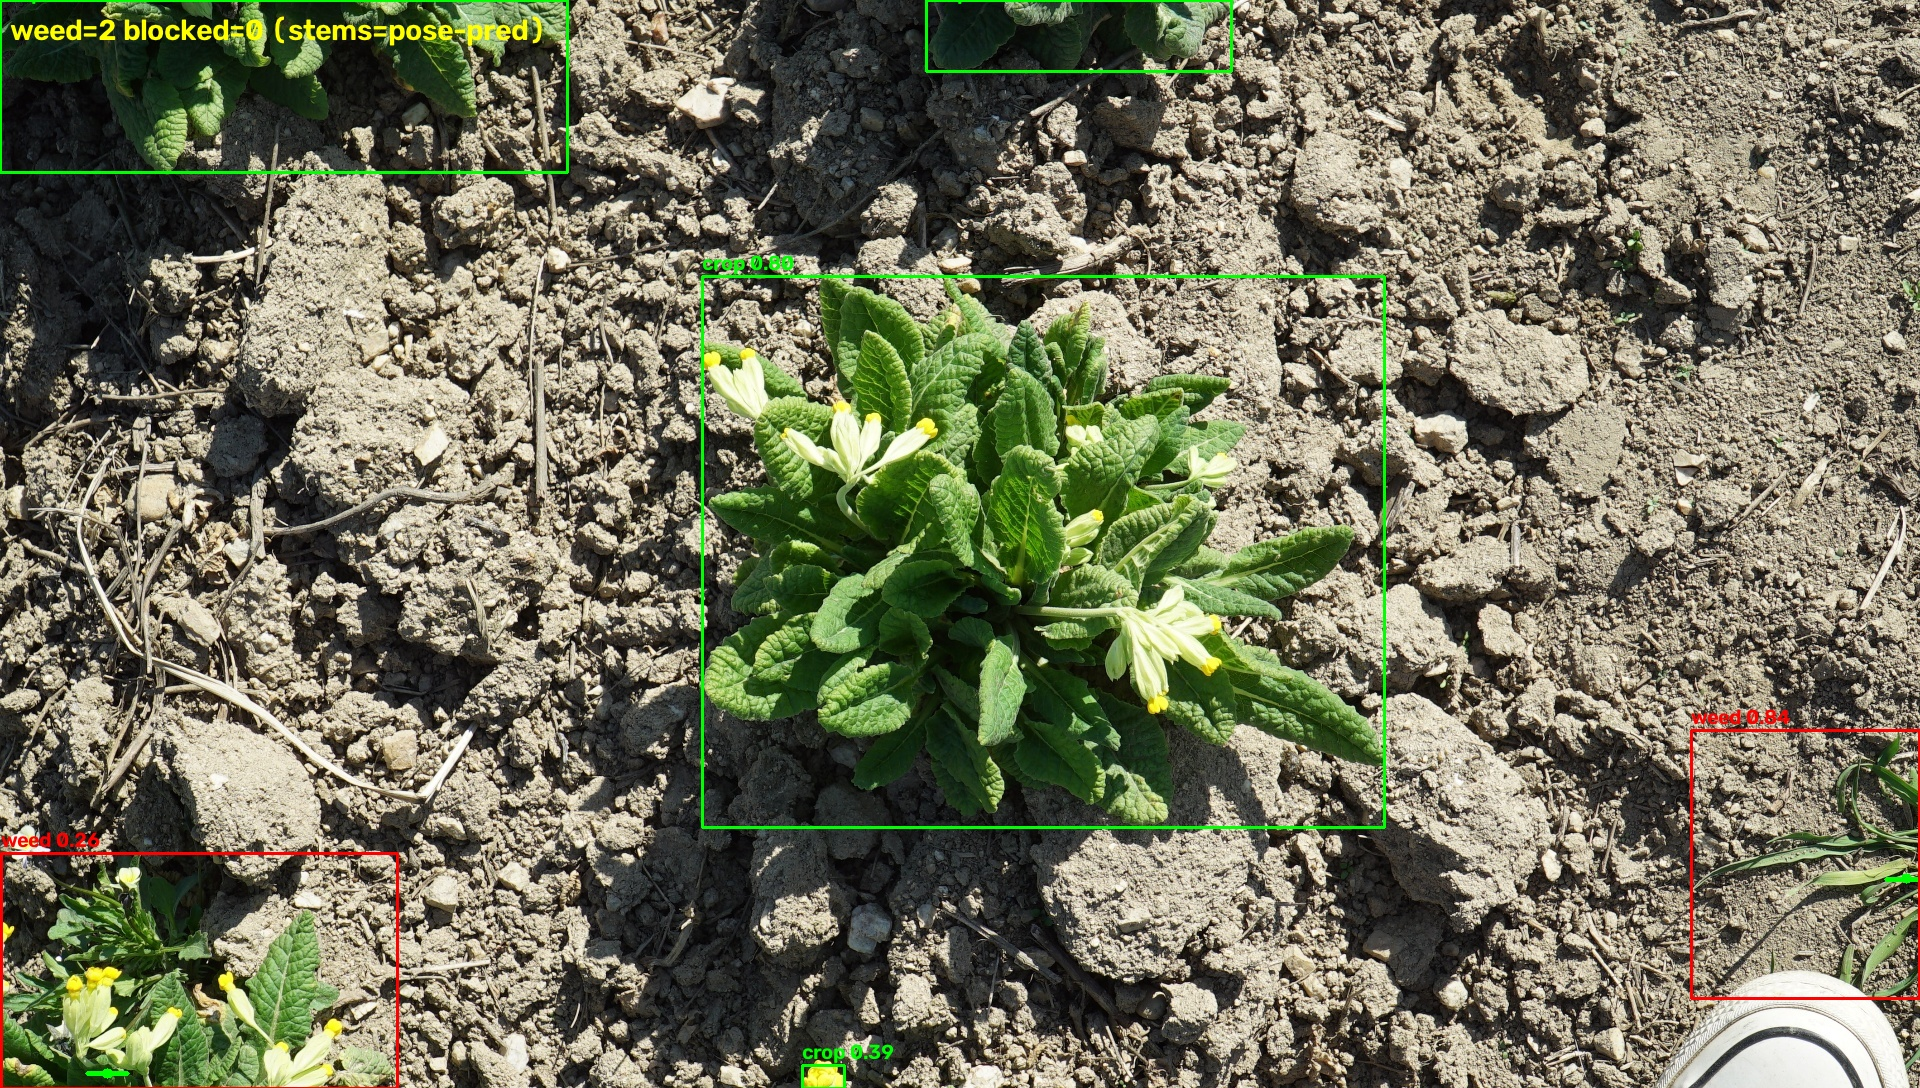
\includegraphics[width=0.88\linewidth]{images/ave-0035-0018.jpg}
\caption{姿态模型（pose）样例：茎点由 YOLO11n-pose 模型预测（而非 GT），切割短线落于预测茎点。}
\end{figure}

% ======================================================================
\section{风险与后续计划}

\begin{enumerate}[label=\textbf{(\arabic*)}]
  \item \textbf{手眼标定（最大风险）}：像素坐标 $\to$ 激光振镜/机械臂坐标的刚体变换，随震动/温漂失效需定期重标定，应尽早排入计划。
  \item \textbf{茎点精度}：数据集茎点多为框中心，真机精确切茎基部需自标关键点微调。
  \item \textbf{深度相机选型}：户外强光下结构光失效，农田宜选双目立体（ZED/OAK-D）或 ToF。
  \item \textbf{seg 模块}：当前作物 mask 使用 GT，需训练 YOLO11-seg 替换为模型预测，完成真正端到端。
  \item \textbf{许可证}：CropAndWeed 非商用，仅限研究/实验。
\end{enumerate}

\vfill
\begin{center}
\small 报告由 Tectonic（XeTeX）自动生成，随训练结果持续更新。
\end{center}

\end{document}
